\paragraph*{2.1 Параметры Денавита-Хартенберга\\}

\hspace*{\parindent}Как известно, для определения любого трехмерного тела в пространстве достаточно задать ему 6 координат (3 координаты перемещения и 3 координаты вращения). Для оптимизации задачи описания положения тела, существует метод, позволяющий сократить число необходимых координат до 4 - метод Денавита - Хартенберга.\\

\hspace*{\parindent}Координаты, позволяющие описать положение тела данным методом называются параметрами Денавита-Хартенберга:
\begin{enumerate} 
% Это не координаты, параметры. Мне кажется слово координаты нужно убрать. Не уверен в правильности употребления по осям, лучше вдоль
 \item[1.] Координатами $a_i$ - обозначаются расстояния по осям $x_i$ (текущая ось) от  $z_{i-1}$ до $z_i$;
 \item[2.] Координаты $\alpha_i$ - обозначают угол вращения оси $x_i$ (текущая ось) от  $z_{i-1}$ до $z_i$;
 \item[3.] Координатами $d_i$ - обозначаются расстояния по осям $z_{i-1}$ (предыдущая ось) от  $x_{i-1}$ до $x_i$;
 \item[4.] Координаты $\theta_i$ - обозначают угол вращения оси $z_{i-1}$ (предыдущая ось) от  $x_{i-1}$ до $x_i$.\\
 \end{enumerate}
 
 \paragraph*{Определение систем координат\\}
 % "В каждом звене" лишнее
\hspace*{\parindent}Для удобного определения осей в каждом звене есть несколько правил:
\begin{enumerate} 
\item[1.] Ось $z_i$ выбирается как сонаправленная с осью вращения $i+1$ сочленения. Далее расположение смежных звеньев будет определяться именно положением этой оси.
\item[2.] Для оси $x_i$ существуют два условия: ось $x_i$ перпендикулярна оси $z_{i-1}$ и пересекает её при мысленном продолжении. (Для упрощения задачи желательно, чтобы в начальных(нулевых) конфигурациях оси $x_{i-1}$ и $x_i$ были сонаправлены.)
\item[3.] Ось $y_i$ задается согласно принципу правой тройки векторов, чтобы выполнялось тождество ($y_i = z_i x x_i$).
 \end{enumerate}

\begin{center}
    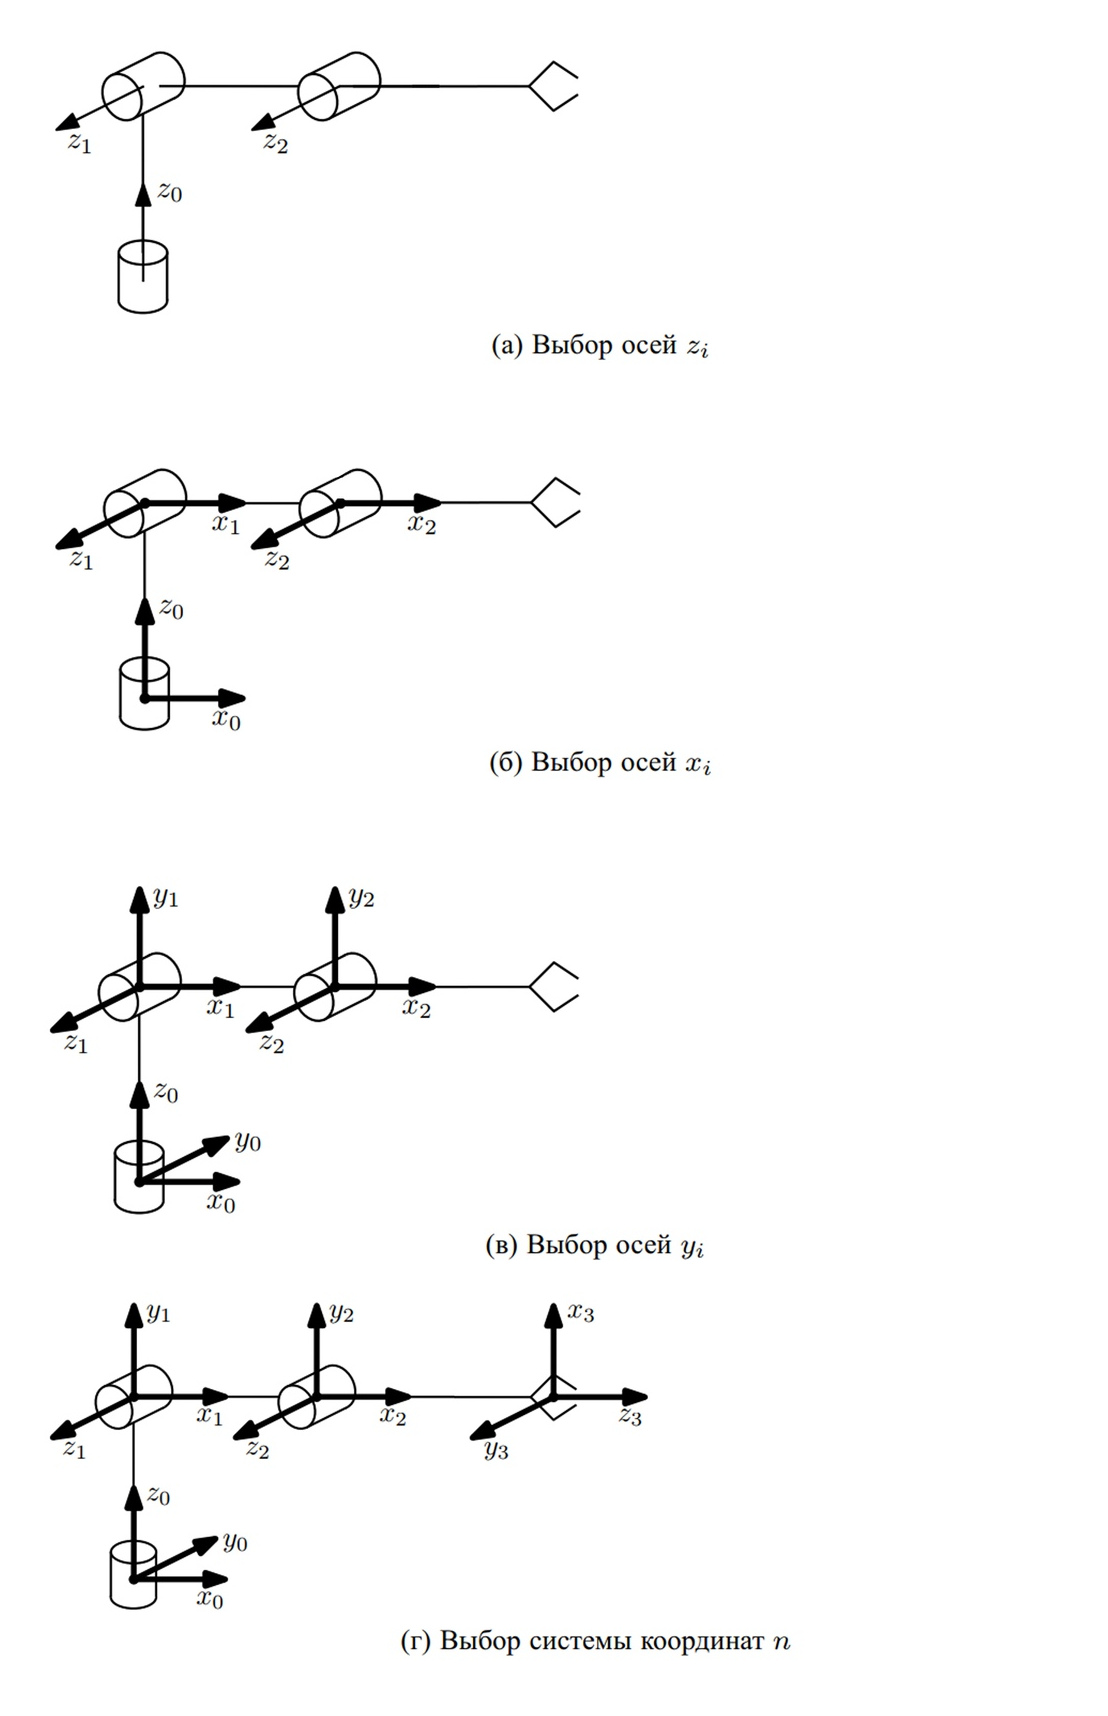
\includegraphics[width=0.8\textwidth]{axes0.jpg}\\
    Рисунок 2.1.1 Определение осей и систем координат.
\end{center}

\hspace*{\parindent}Как ранее говорилось, сперва выбираются значения осей $z_i$: ось вращения первого звена будет проходить через ось изображаемого цилиндра, т.к. вращение происходит в этой плоскости, аналогично выбираются оси для остальных звеньев вращения, также можно заметить, что можно было выбрать направление осей $z_1$ и $z_2$ "от нас", но это  ухудшает наглядность схемы, поэтому выбирается направление "на нас". Оси $x_i$ выбираются по принципу перпендикулярности к соответствующим осям $z_i-1$, и направленные на пересечение с последующими из них, так выбрано направление "вправо" в первом звене и сонаправленном с ним втором для нулевого параметра начального угла в параметрах DH. Далее происходит смещение только по оси перпендикулярной оси вращения, поэтому направление осей $x_i$ остаётся неизменным. Оси $y_i$ достраиваются в соответствии с правилом правой тройки векторов (можно использовать и левую, что приведёт к некотором изменениям знаков в дальнейших преобразованиях, но наиболее используемой является правая). Система последнего звена получается путём смещения на некоторое расстояние, поскольку схват и его сочленения статичны.\\
 
 \paragraph*{Пример\\}
 
\hspace*{\parindent}Рассмотрим нахождение этих параметров на конкретной задаче:\\

Пусть имеется такая система:\\
\begin{center}
    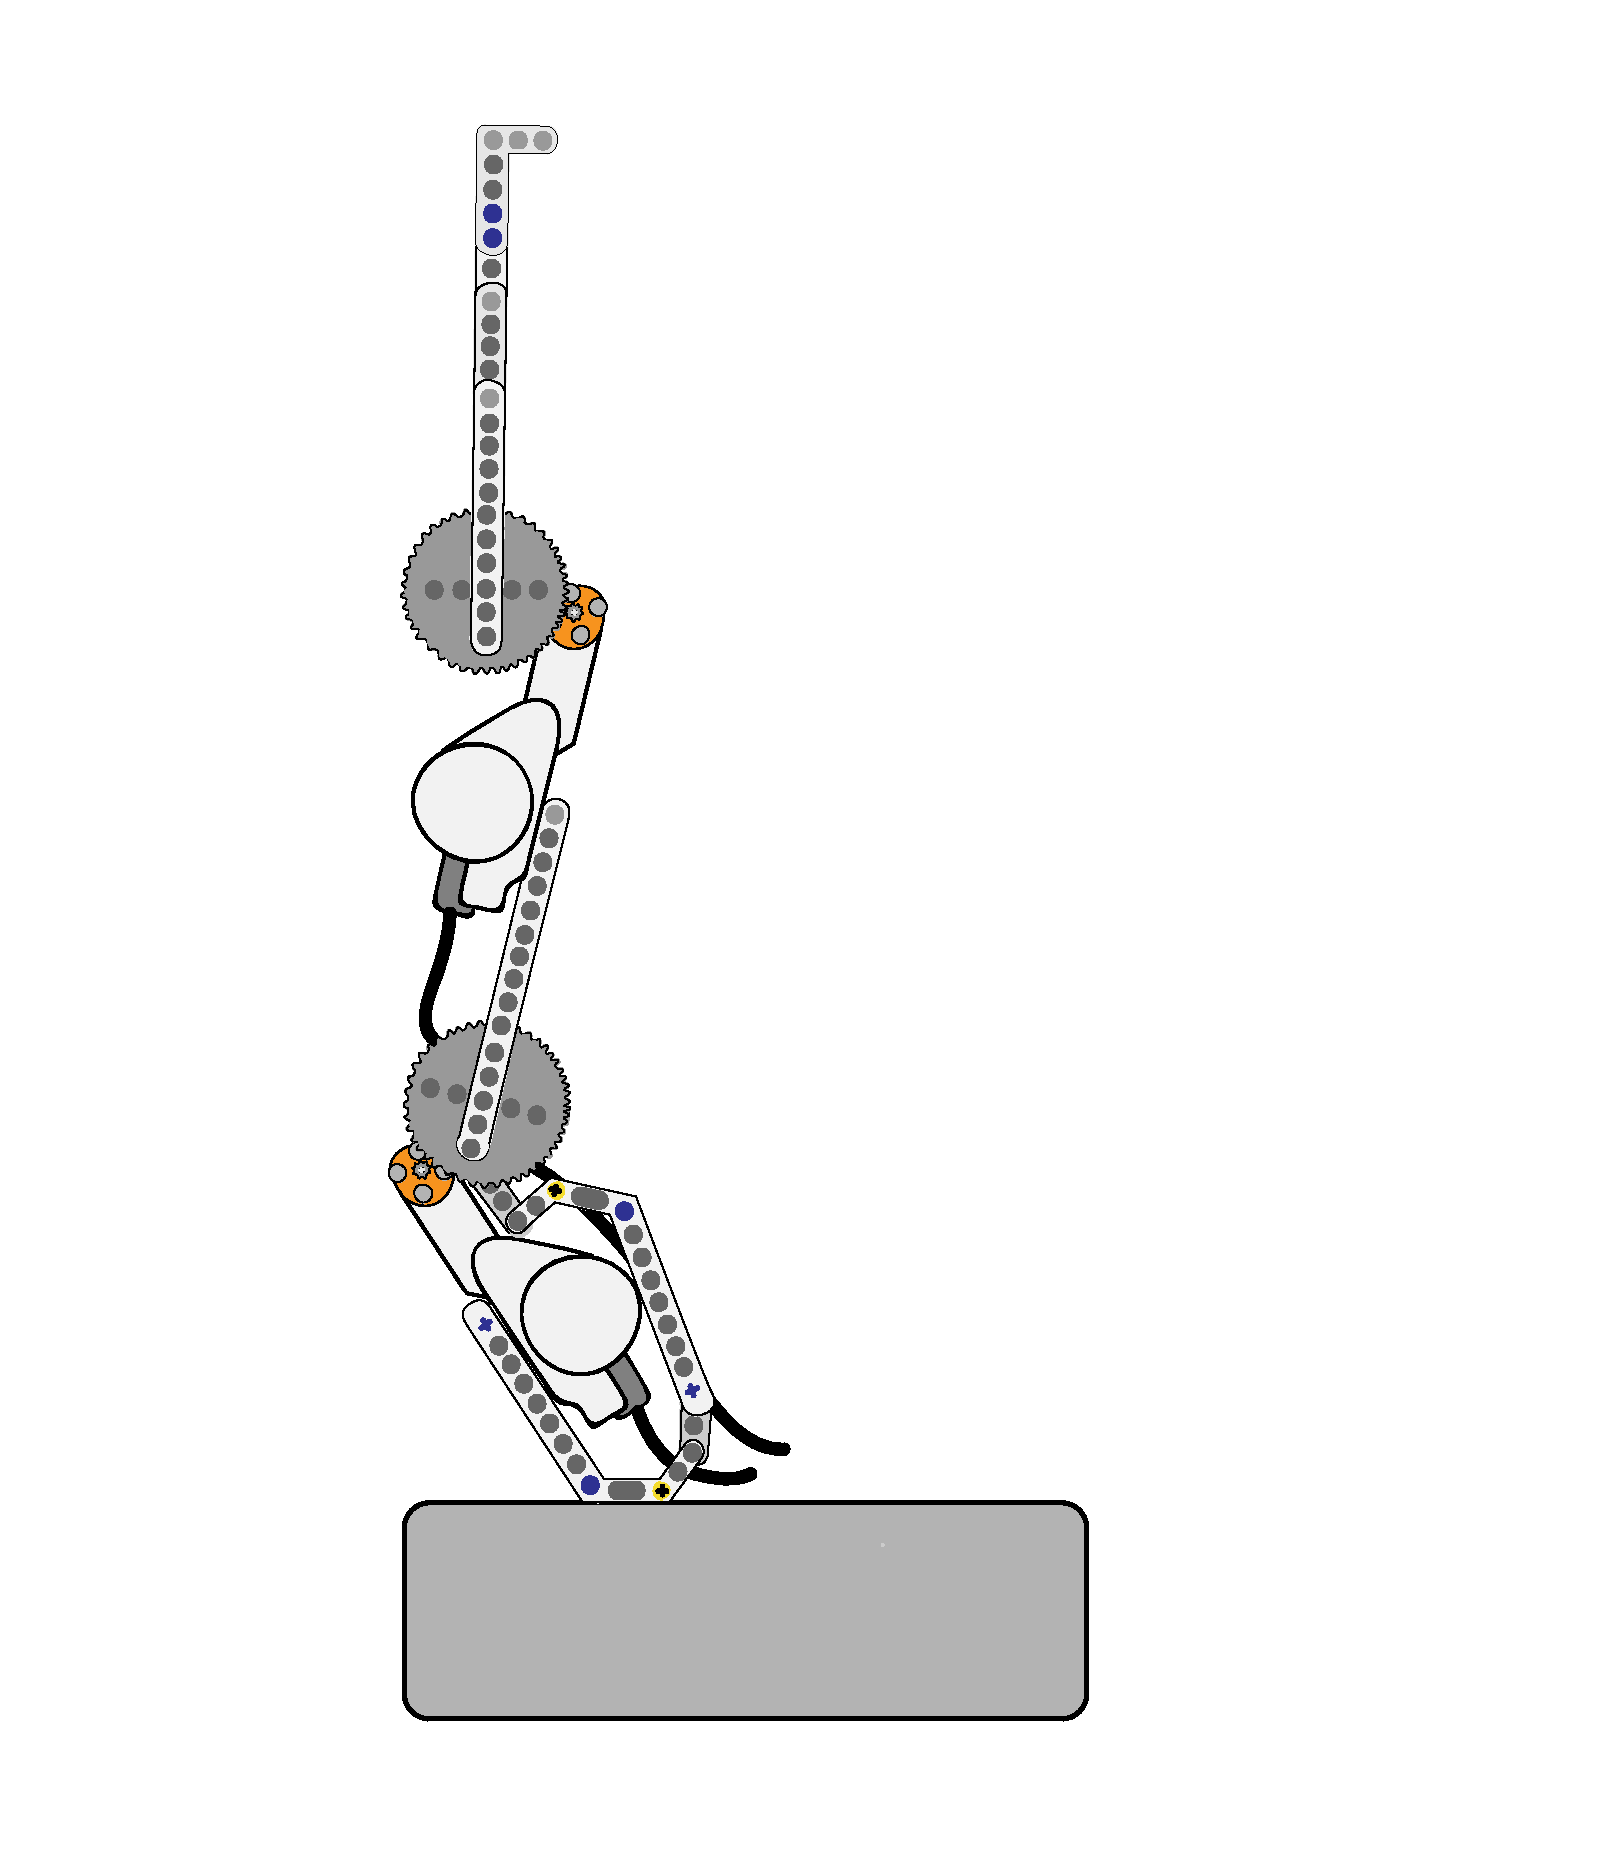
\includegraphics[width=0.6\textwidth]{DH1.pdf}\\
    Рисунок 2.1.2 Система для определения DH параметров.\\
\end{center}


\hspace*{\parindent}Расставляются положения DH-параметров по правилам, описанным выше:\\ 
\hspace*{\parindent}В начале определяются параметры $a_i$: системы $x_0y_0z_0$ и $x_1y_1z_1$ совпадают, следовательно сдвигов нет, далее рассматривается пара систем $x_1y_1z_1$ и $x_2y_2z_2$ здесь ость $z_2$ лежит в плоскости перпендикулярной рассматриваемому виду и располагается в направлении "от нас", её нулевая координата соответственно совпадает с нулевыми координатами $x_2$ и $y_2$, а значит $a_1$ определяется как расстояние от пересечения $x_1z_1$ до  $x_2y_2$ по оси $x_2$, следующее смещение между осями $z_2$ $z_3$ и $z_3$ $z_4$ выполняется аналогично, они направлены "от нас" и лежат в перпендикулярной плоскости, их начала лежат на пересечении двух других осей, соответственно получаются значения $a_2$ и $a_3$.\\
\hspace*{\parindent}Далее коэффициенты смещения $d_i$: имеется только смещение $d_1$ (поскольку остальные системы по осям $z_i$ не имеют сдвигов) от первой системы до второй.\\
Углы $\alpha_i$ определяются как поворот текущей оси $x_i$ от оси $z_{i-1}$ до оси $z_{i}$. Например, для первого звена ось $z_0$ направлена вверх, а $z_1$ от нас. Значит, поворот был на угол $\frac{\pi}{2}$. \\
\hspace*{\parindent}Углы $\theta_i$ определяются как углы вращения на сочленениях: можно заметить, что при переходе от первой системы ко второй производится дополнительный поворот на угол $\frac{\pi}{2}$, что также заносится в параметр, остальные углы подобного дополнительного вращения не имеют.\\
\begin{center}
    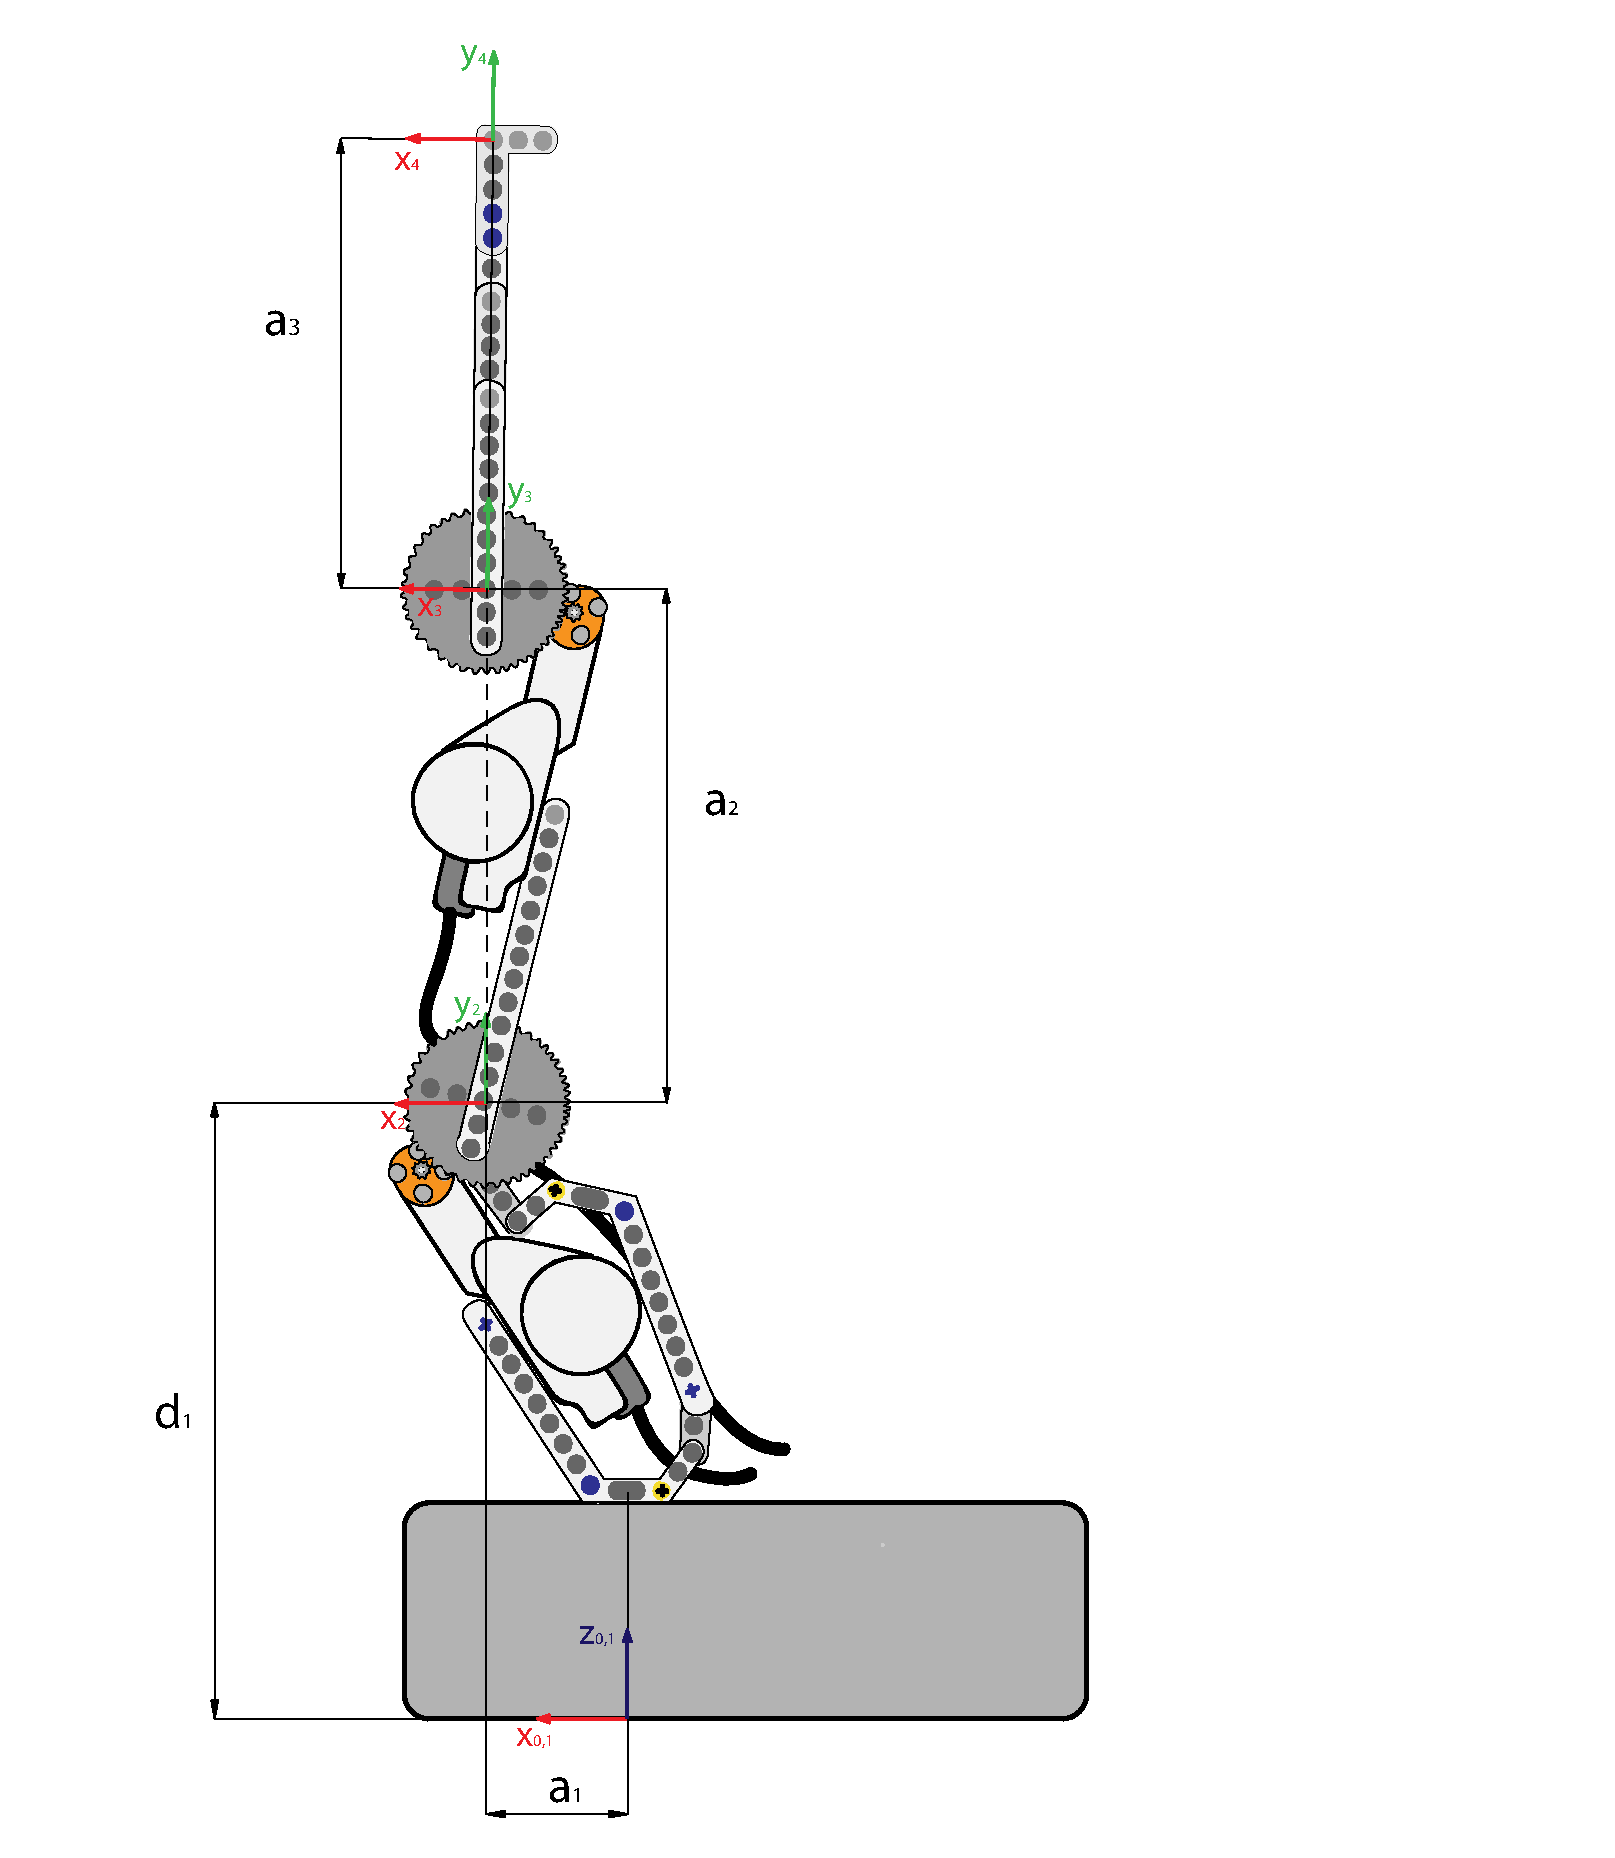
\includegraphics[width=0.575\textwidth]{DH2.pdf}\\
    Рисунок 2.1.3 Система с обозначенными DH параметрами.\\
\end{center}



\begin{table}[h!]
\hspace*{\parindent}Далее измеряются их значения и заносятся в соответствующую таблицу:\\
\begin{center}
\begin{tabular}{|c|c|c|c|c|}
\hline
Звено i & $a_i$ & $\alpha_i$ & $d_i$ & $\theta_i$ \\
\hline
1 & 0,06 & $\frac{\pi}{2}$ & 0,163 & $\theta_1$\\
\hline
2 & 0,15 & 0 & 0 & $\theta_2$ + $\frac{\pi}{2}$\\
\hline
3 & 0,145 & 0 & 0 & $\theta_3$\\
\hline
\end{tabular}
\end{center}
\end{table} 

\newpage
\hspace*{\parindent}После того, как были получены значения, достаточные для описания положения тела в пространстве, можно приступать к задачам нахождения связи между обобщенной системой координат манипулятора и системы координат, связанной со схватом (рабочим инструментом). Для этого будут использованы матричные преобразования систем координат.\\

